Fido was implemented in the C++ programming language with minimal use of the standard library.
This was to enable cross-platform functionality, lightweight and speedy performance, and the ability to run on microcontrollers if necessary.
In order to test Fido both a simulation environment and three hardware implementations were constructed and written driver suites for interaction with inputs and outputs.

\subsection{Simulation}

An asynchronous simulator was created using C++ and the SFML graphics library in order to efficiently test Fido's performance on different types of robots.
Multiple inputs were modeled for simulation with outlets for control both by a human operator using sliders and by programmed handlers using a bridge class.
Sensors included a microphone, light sensor, infrared light sensor, inertial measurement unit, and three axes of radio receivers allowing measurement from a radio beacon.
Multiple tasks were trained using both operator input and autonomous ``taskmaster'' programs to regulate positive and negative feedback.


\begin{figure}[H]
	\centering
	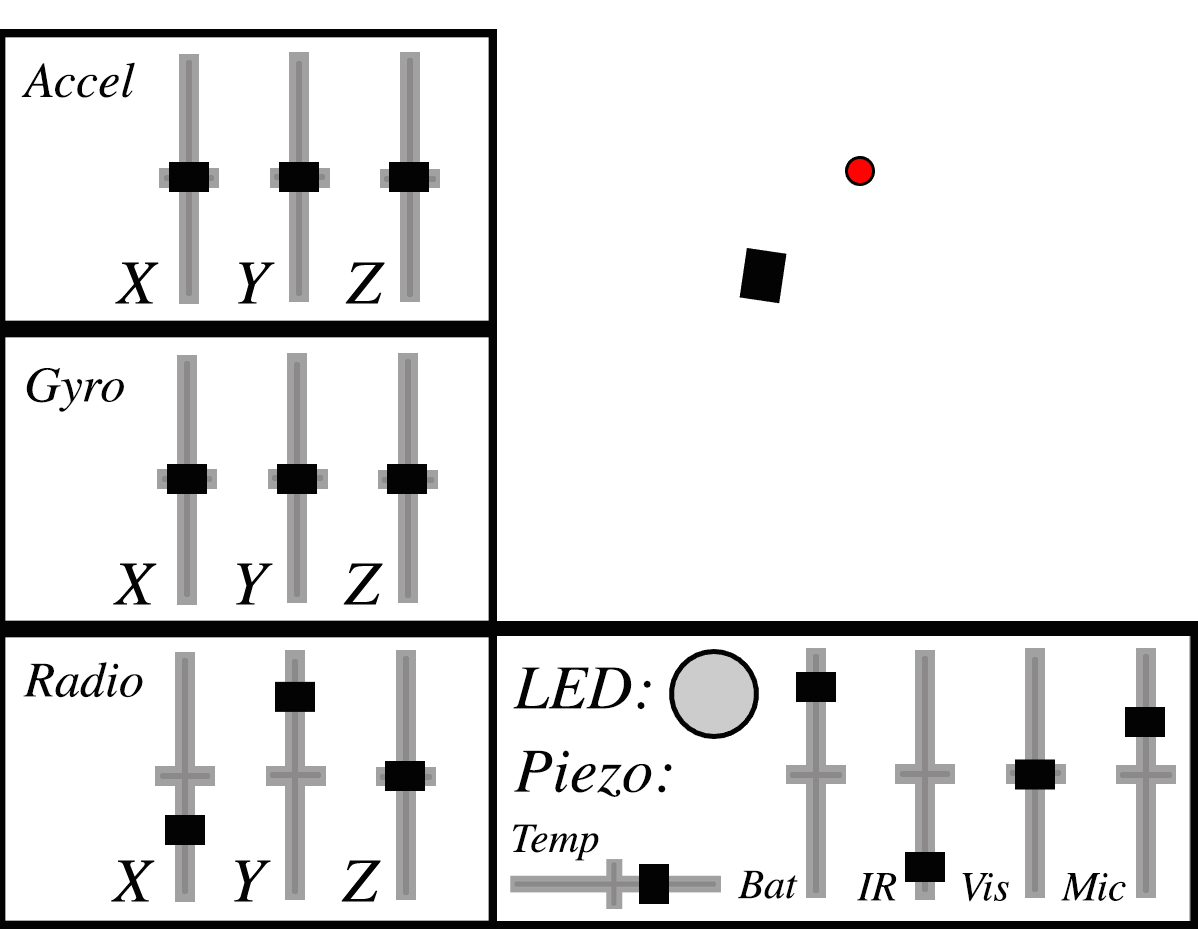
\includegraphics[height=10cm]{Figures/Screenshot.png}
	\caption{Screenshot of the Fido Simulator Graphical User Interface}
\end{figure}

Fido's outputs were chosen similarly.
A buzzer of varying tone and frequency can play sounds and a multicolor LED can be lit to any red-green-blue color combination.
Two motors allow movement using one of two kinematic configurations: differential drive similar to that of a tank, or holonomic control for each axis of movement.
Appropriate kinematics for each model including acceleration and friction were implemented with help from \cite{dudek}.

The black rectangle in the upper right corner of the simulator is the robot, having been moved as part of training.
The red dot near the rectangle is a graphical representation of a radio beacon.
As adjusting sliders to represent the location of a radio beacon relative to the robot would be impractical, we decided to implement a beacon that could be placed and dragged by right clicking on the simulator.
Simulated sensor readings of beacon strength on two axes are gathered using an inverse square law, as applies to radio waves in general.
These readings are then displayed in the sliders and can be manually altered as well.
The radio beacon can be removed by a human operator by pressing the ``p'' key in the simulator environment.
This was especially helpful in the task of training Fido to follow a radio beacon.

\subsection{Hardware Implementations}

Three hardware implementations were next constructed to test Fido's real world trainability, universality, and applicability.
In order to facilitate this, the three robots were designed to have vastly different kinematics and functionality.
The robots, nicknamed ``Thing One,'' ``Thing Two,'' and ``Thing Three,'' all ran on embedded GNU/Linux systems and were trained via a cross-platform mobile application over Wi-Fi.

\subsubsection{Thing One}
\begin{figure}[H]
	\centering
	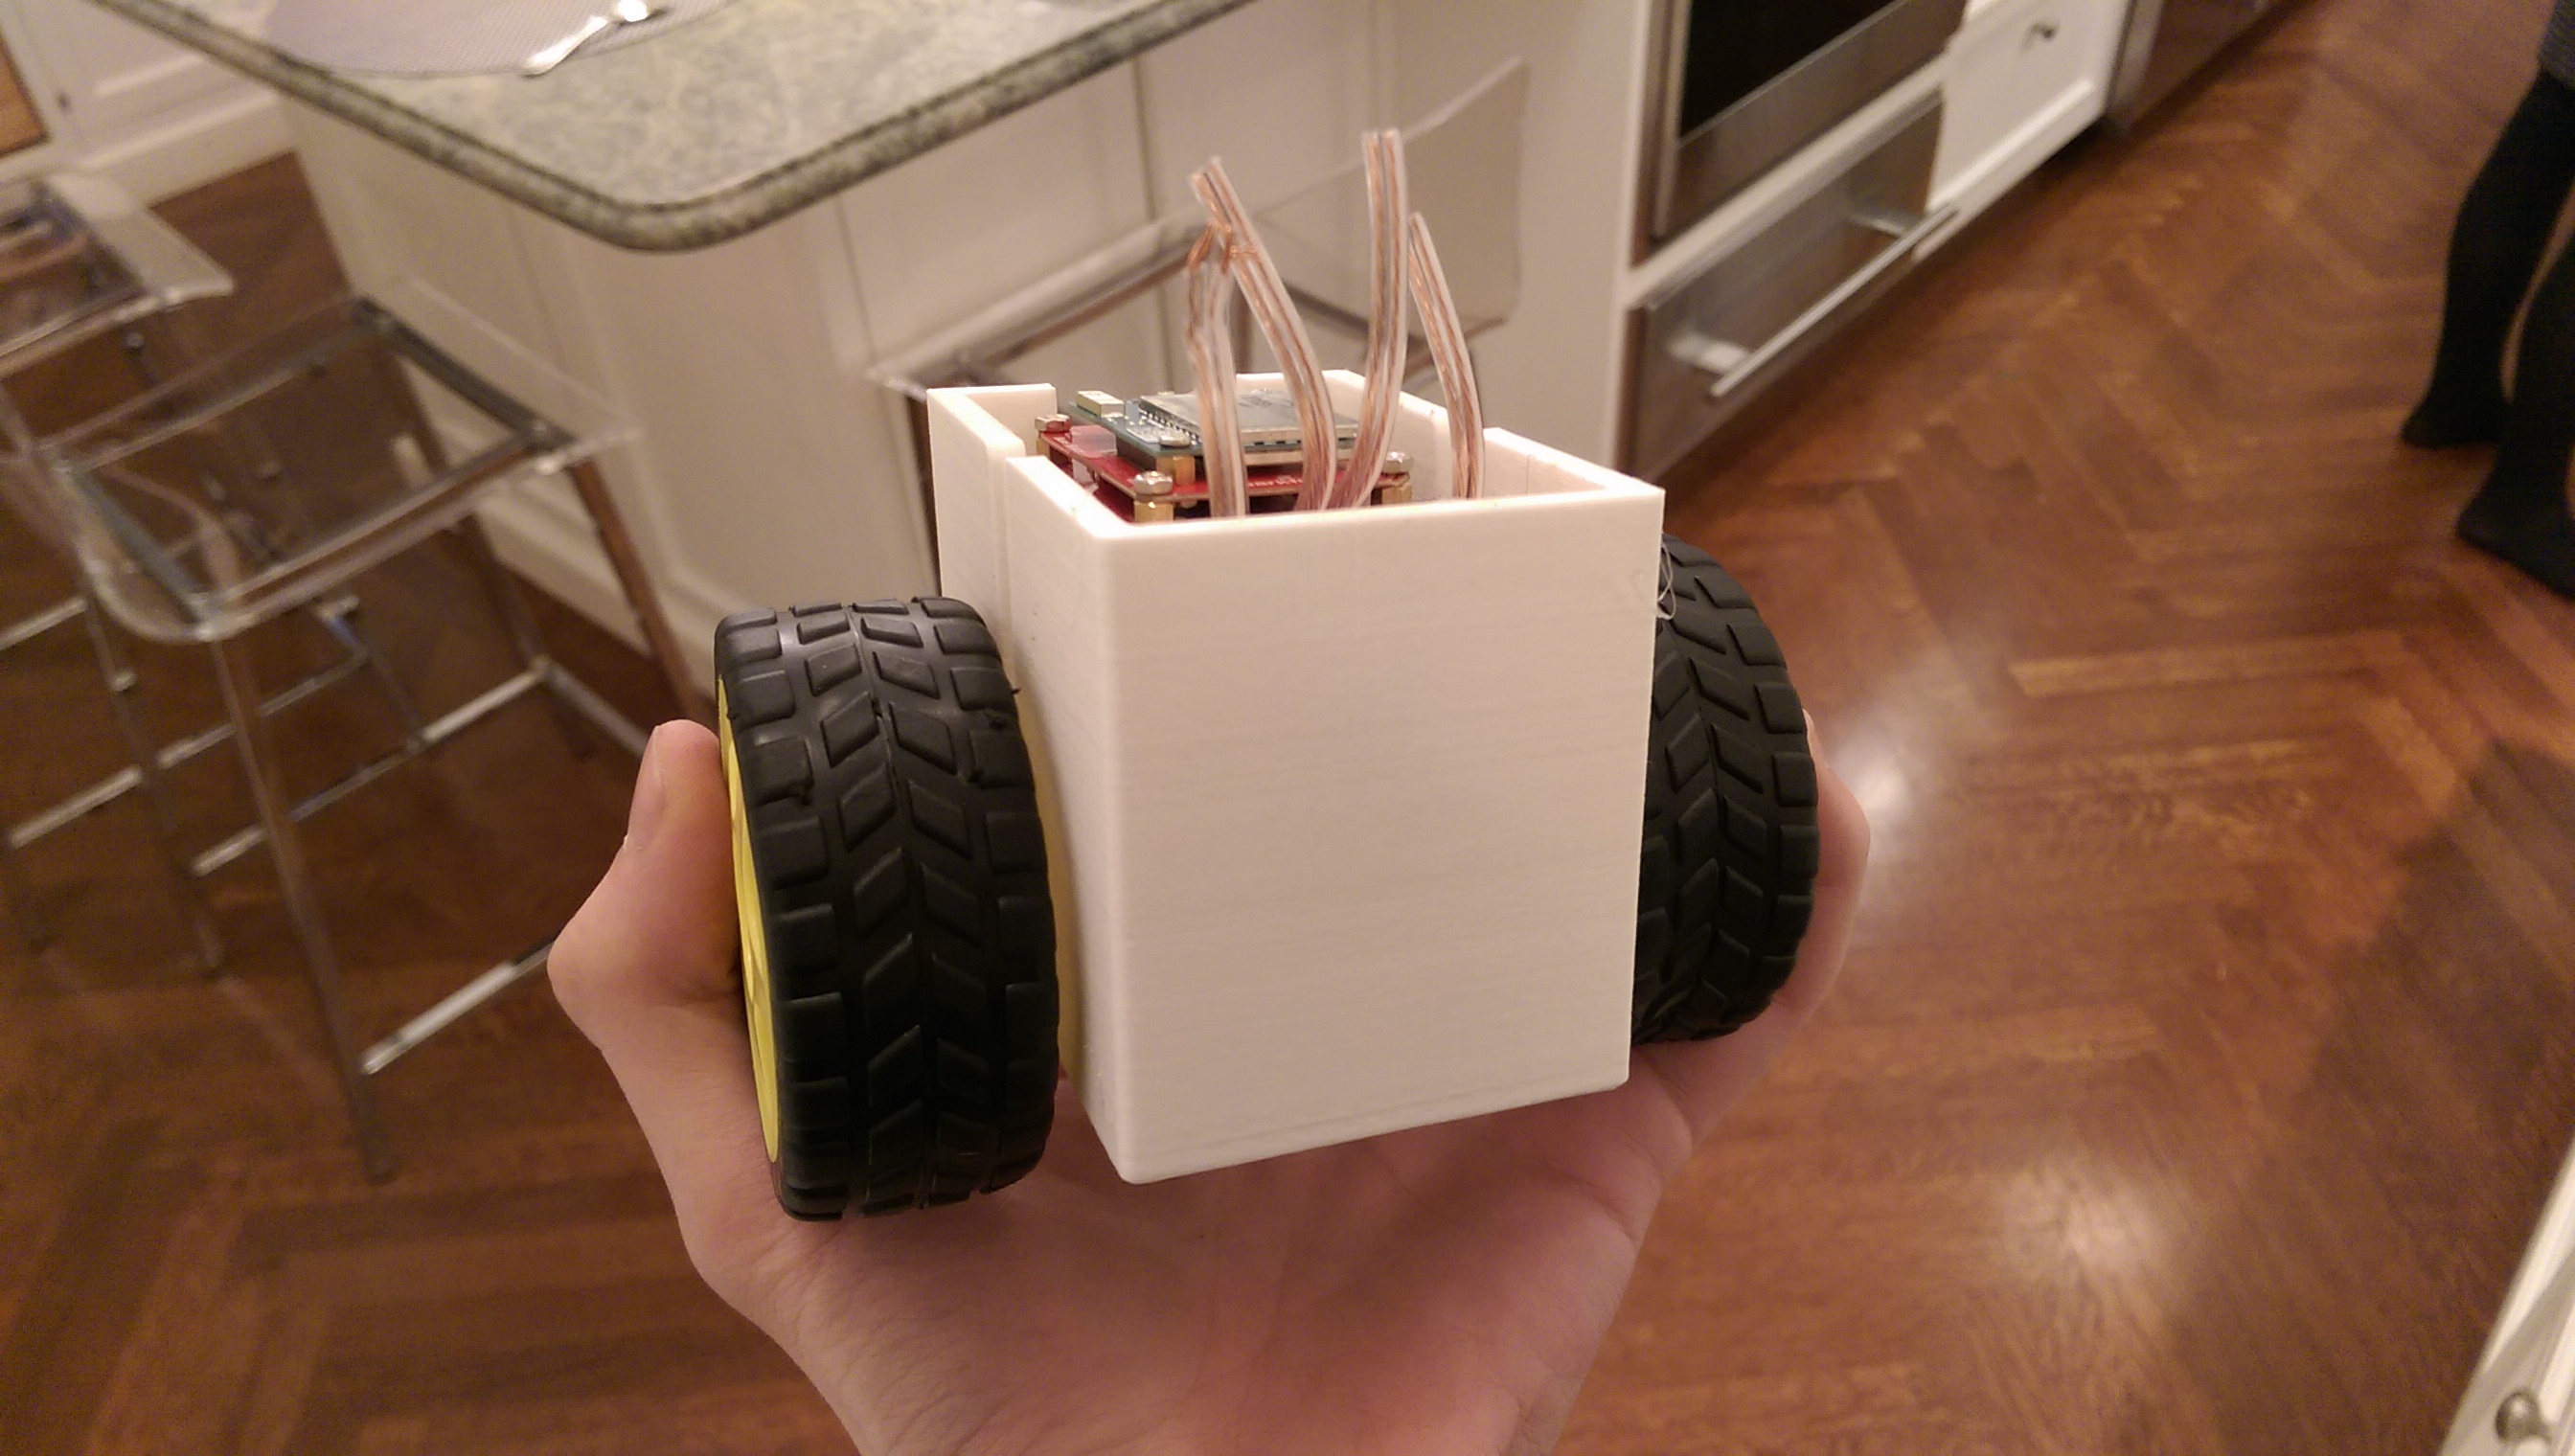
\includegraphics[height=6cm]{Figures/Prototype.jpg}
	\caption{Fido Thing One with Head-Cap Removed}
\end{figure}

The first hardware implementation constructed, nicknamed ``Thing One,'' consisted of an Intel Edison GNU/Linux Single Board Computer, a two-wheeled differential drive system, and a 3D-printed case.
The implementation was given an ambient light sensor, an inertial measurement unit, and a microphone as inputs, with its two motors as outputs.
A differential drive system was chosen due to its standardization in the field, while the Intel Edison was chosen due to its low power consumption and integrated wireless networking capabilites.

\subsubsection{Thing Two}
\begin{figure}
	\centering
	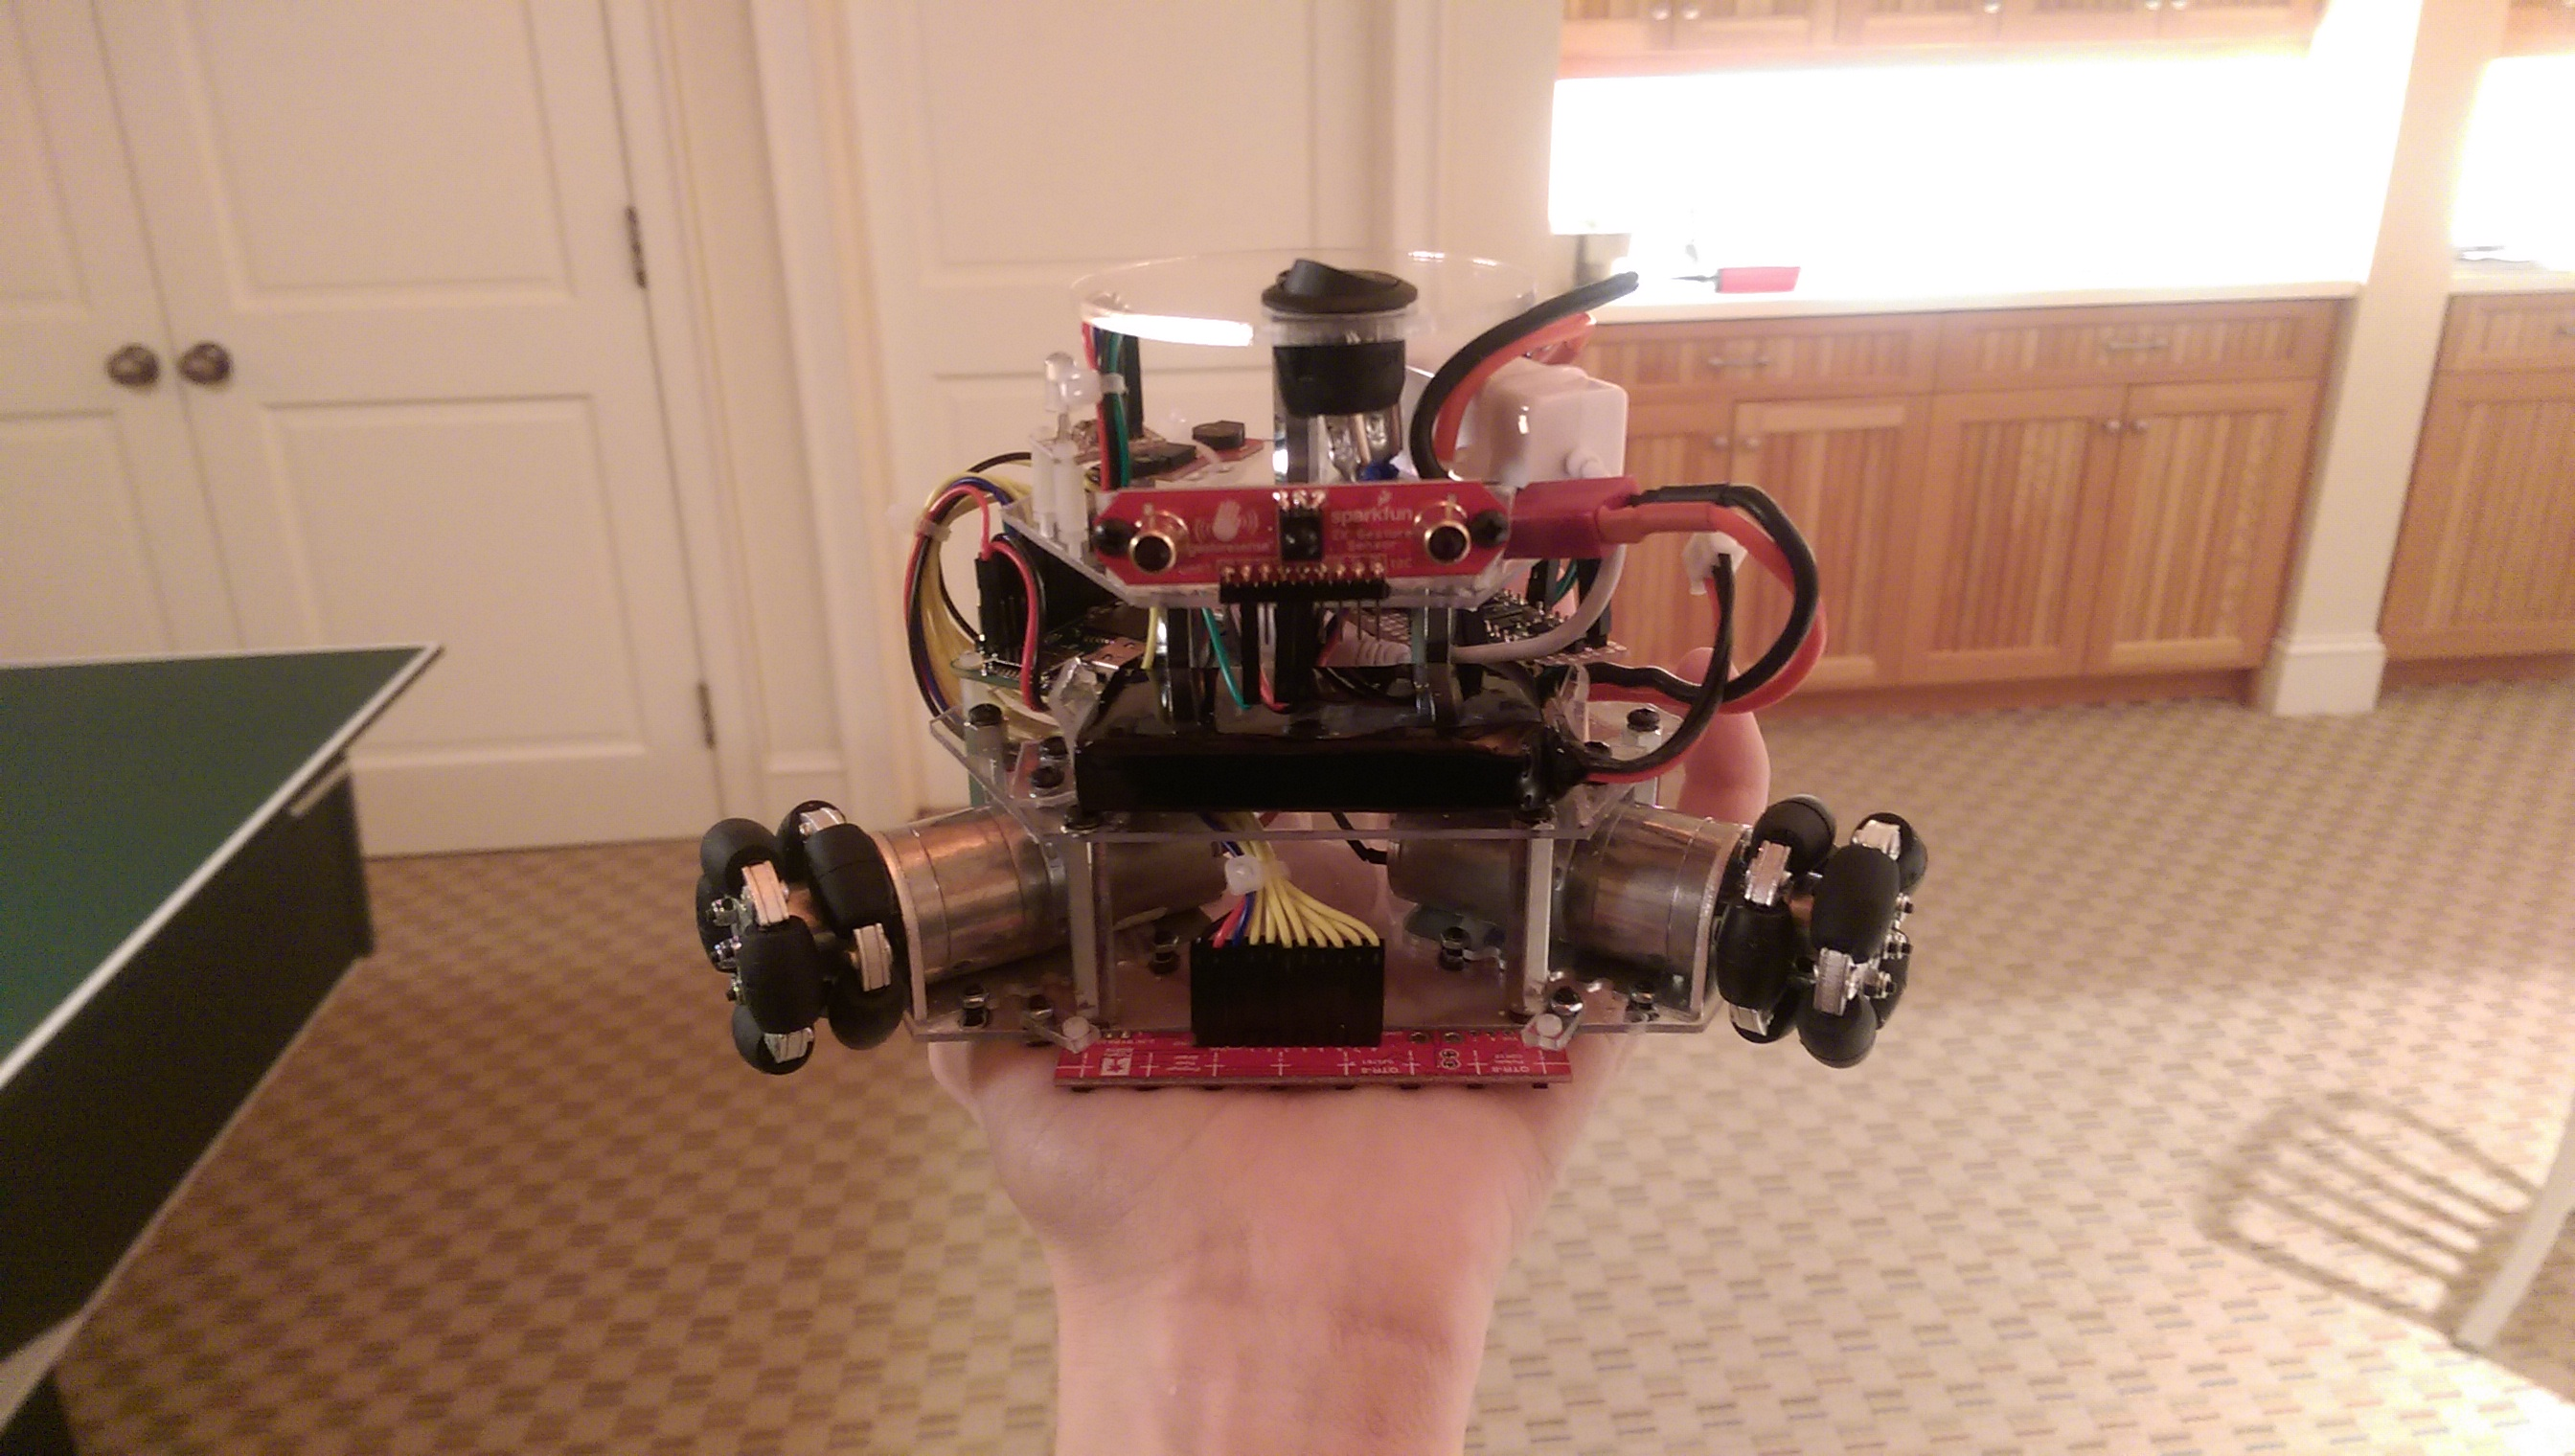
\includegraphics[height=6cm]{Figures/ThingTwo.jpg}
	\caption{Fido Thing Two}
\end{figure}

The second hardware implementation to be constructed was named ``Thing Two,'' and utlized a three 90$^{\circ}$ Swedish wheel holonomic drive system.
This more complex drive system challenged the Fido control system with the advanced kinematics neccesary to manipulate the system in every possible degree of freedom.
The robot was powered by the \$5 Raspberry Pi Zero, demonstrating that Fido could be run on lower cost and power hardware.
The body was cut from 1/8\" polycarbonate and bolted together using hex standoffs to create a tiered structure for mounting various sensors and electronics.
The inputs to the system were a ZX gesture sensor, a line following infrared array, an inertial measurement unit and an ambient RGB color sensor.
The outputs from the system were its three motors, a piezoelectric buzzer, and an RGB light-emitting diode.

\subsubsection{Thing Three}
\begin{figure}
	\centering
	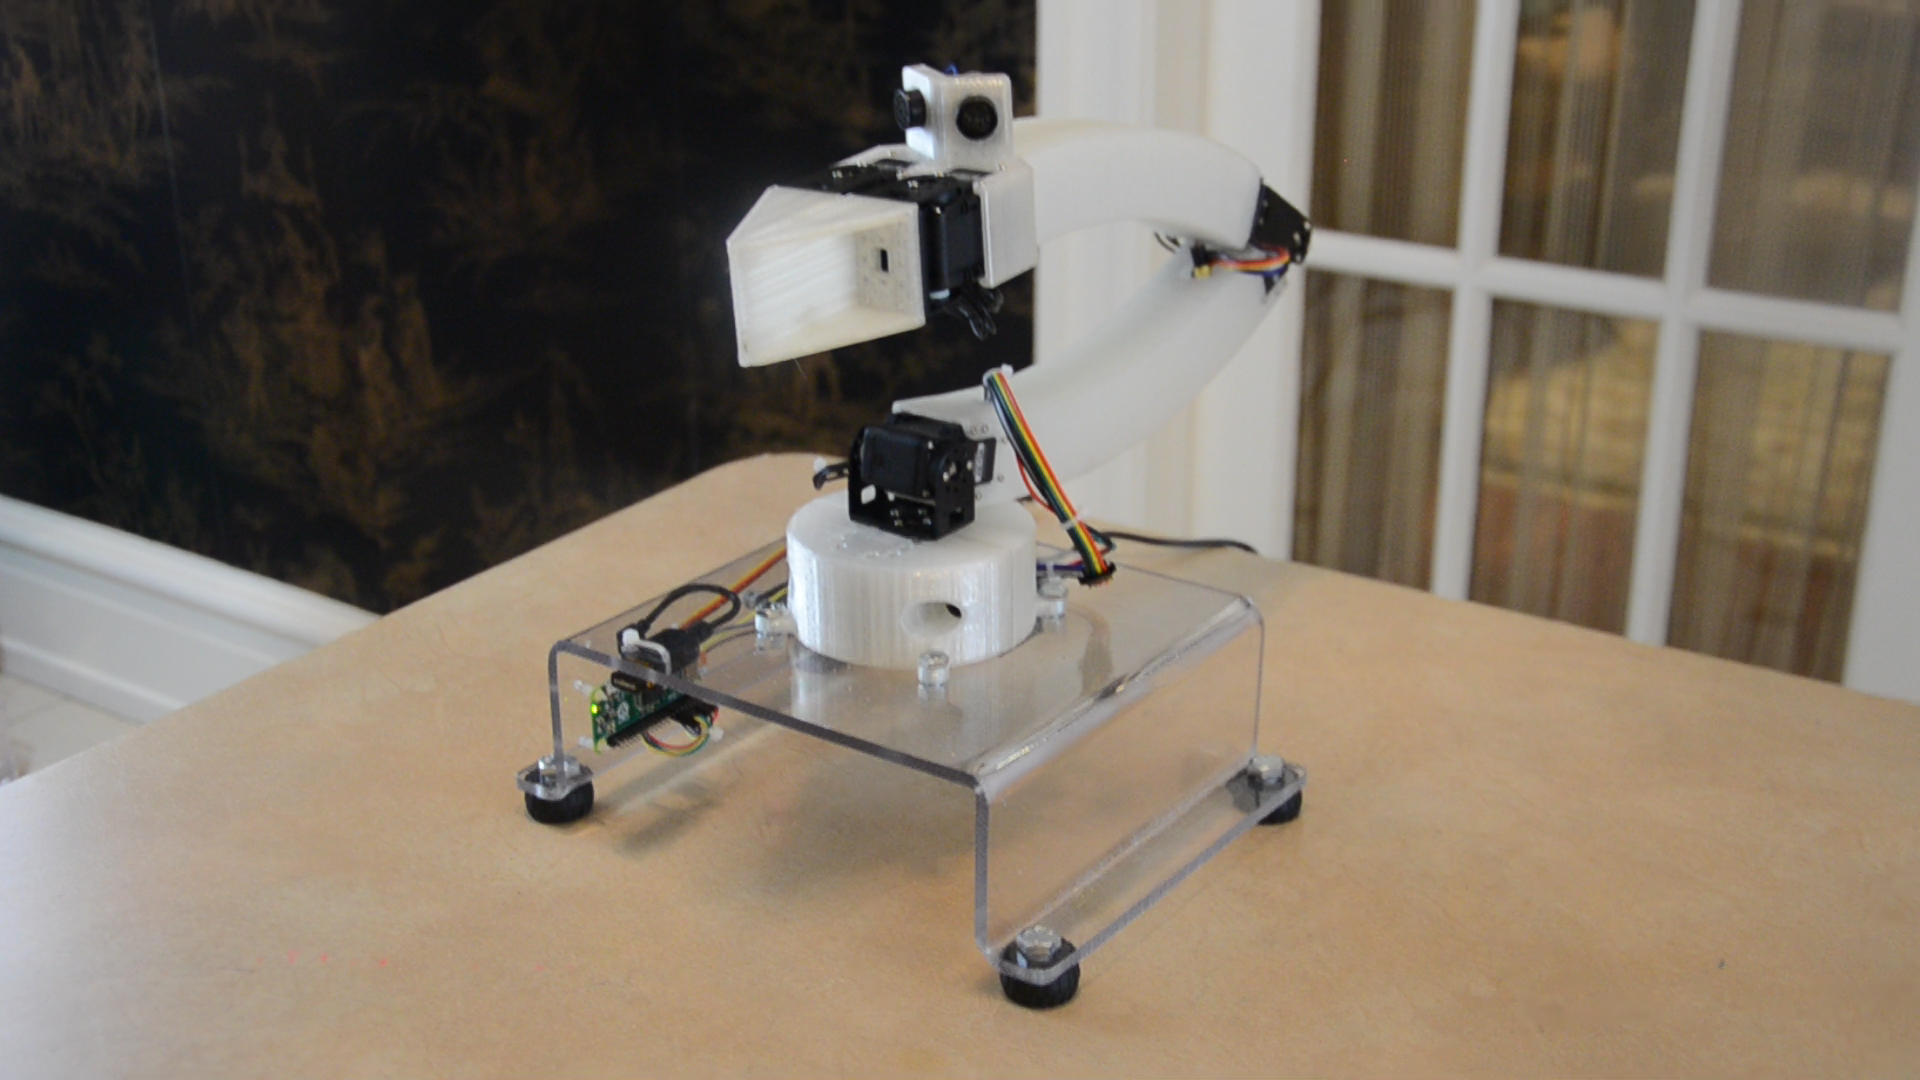
\includegraphics[height=6cm]{Figures/ThingThree.png}
	\caption{Fido Thing Three}
\end{figure}

The third and final hardware implementation constructed was a four axis robotic arm nicknamed ``Thing Three.''
A departure from the wheeled mobile robots previously detailled, Thing Three was created to demonstrate Fido's extensive universality and applicability in practical settings.
The robot's chassis was 3D printed out of translucent PLA plastic, with a hollow interior for wire and LED strip routing.
The LED strip was used to indicate reward administration during training.
The arm was actuated by five Dynamixel AX-12A servo motors, and controlled by a Raspberry Pi Zero.
The inputs to the system were two MaxSonar ultrasonic sensors and the arm's joints' current positions, while its outputs were its servo motors and LED strip.

\subsection{Training App}

\begin{figure}
	\centering
	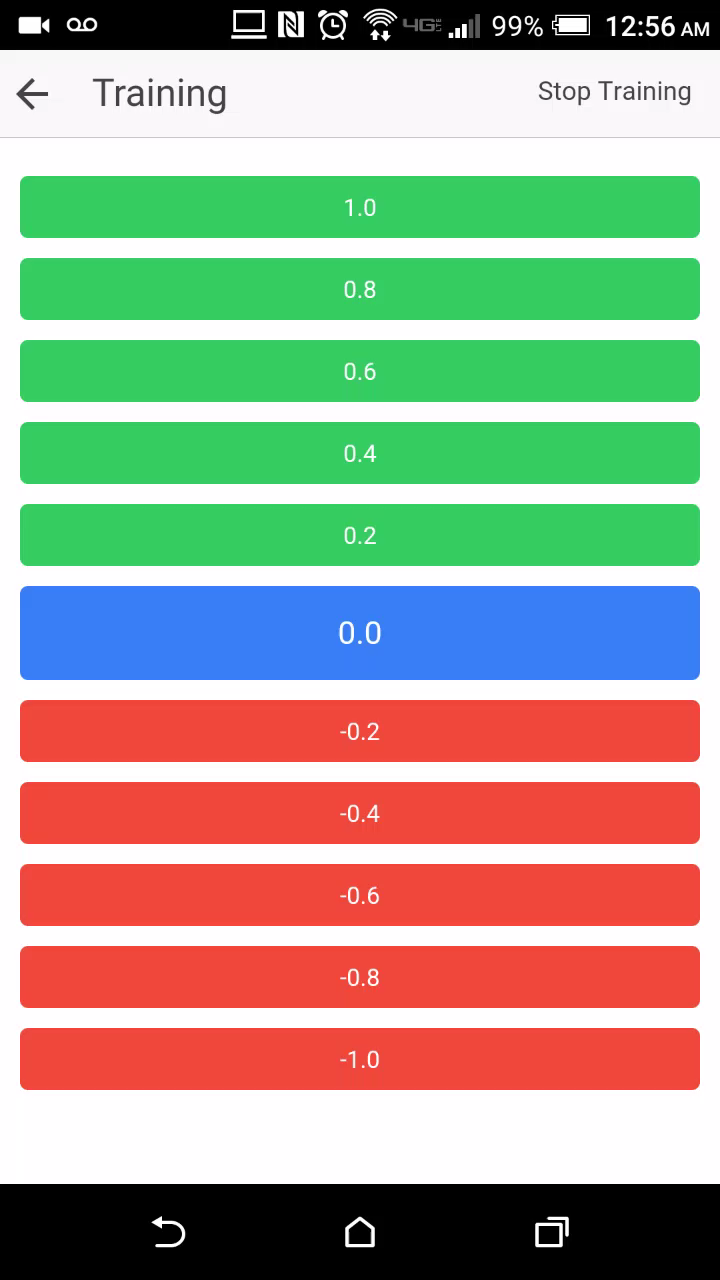
\includegraphics[height=6cm]{Figures/IonicScreenshot.png}
	\caption{Screenshot of the Training App during Robot Training}
\end{figure}

Next, a crossplatform mobile application was created to assist training Fido's hardware implementations.
The application allowed an operator to connect to a hardware implementation over Wi-Fi using TCP sockets, administer reward, and run trained models.
Gradient reward could be administered to the Fido control system from -1 to 1, with positive feedback shown in green and negative feedback shown in red.
The application was developed using web technologies through the Ionic Framework.
